\section{Component View}
\subsection{Database}
The database tier runs MySQL Community Edition and uses InnoDB as storage engine: the DBMS is fully transactional with rollback and commit, besides it ensure ACID properties and provides automatic recovery from crashes via the replay of logs.

The DBMS will not be internally designed because it is an external component used as a “black box” offering some services: it only needs to be configured and tuned in the implementation phase.
The database can communicate only with the business logic tier using the standard network interface, described in section 2.6. 

Security restrictions will be implemented to protect the data from unauthorized access: the database must be physically protected and the communication has to be encrypted.
Access to the data must be granted only to authorized users possessing the right credentials and system privileges allow only administrators to perform administrative actions in the database, including privileges such as: create database, create procedure, create view, backup database, create table, and execute.

Every software component that needs to access the DBMS must do so with the minimum level of privilege needed to perform the operations. All the persistent application data is stored in the database.
The conceptual design of the database is illustrated by the ER diagram.

Foreign key constraints and triggers are not used: the dynamic behaviour of the data is handled entirely by the Java Persistence API in the Business Application tier.

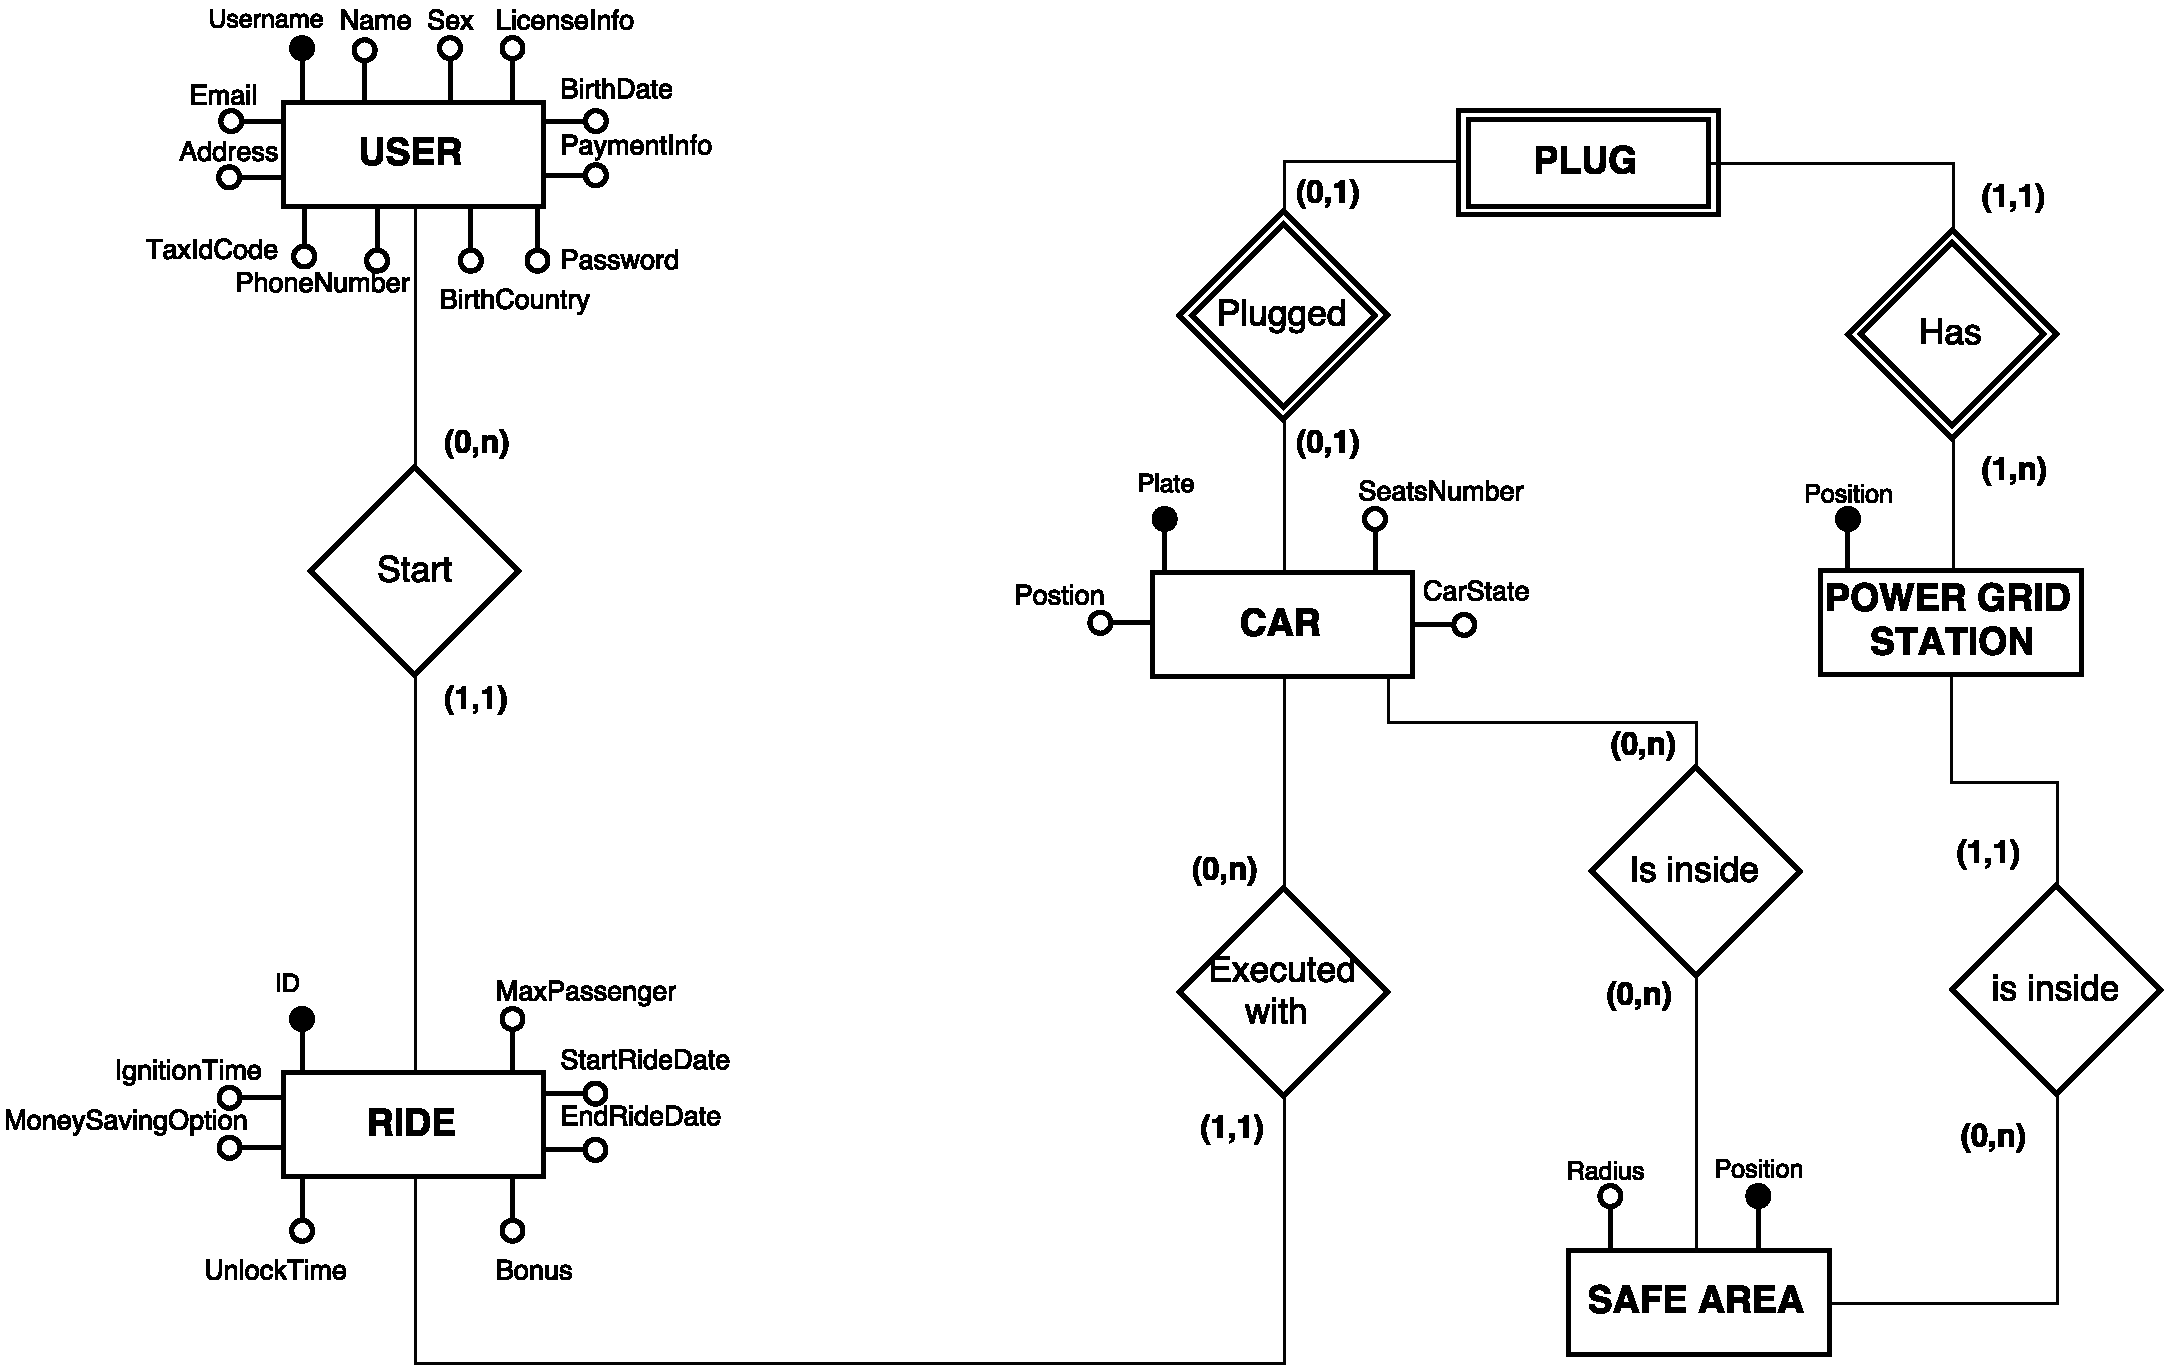
\includepdf{architectural_design/Architecture_Diagrams/ERDiagram.pdf}

\subsection{Application Server}
The application server is implemented in the business logic tier, it runs on an open-source application server, GlassFish, that use Java EE and supports Enterprise JavaBeans.
The access to the DBMS is not implemented with direct SQL queries but using Java Persistence API (JPA), in particular the Java Persistence Query Language (JPQL) makes queries against entities stored in DBMS.
Queries resemble SQL queries in syntax, but operate against entity objects rather than directly with database tables.
The object-relation mapping is done by entity beans.

The Entity Beans representing the database entities are strictly related to the entities of the ER diagram,the data  are stored automatically using container-managed persistence.
They are persistent because their data is stored persistently in the database and they do survive a server failure, failover, or a network failure.
The business logic is implemented by custom-built stateless Enterprise JavaBeans (EJB).

Our application is quite simple, the state of the cars is stored in the DB, so we do not need stateful EJBs which can be more expensive,but just stateless EJBs.
Concurrency management and performance are fundamental, so the reuse of EJBs for many requests is a desirable behaviour.
The application server implements a RESTful API using JAX-RS to allow the clients to use the services offered by the EJBs.
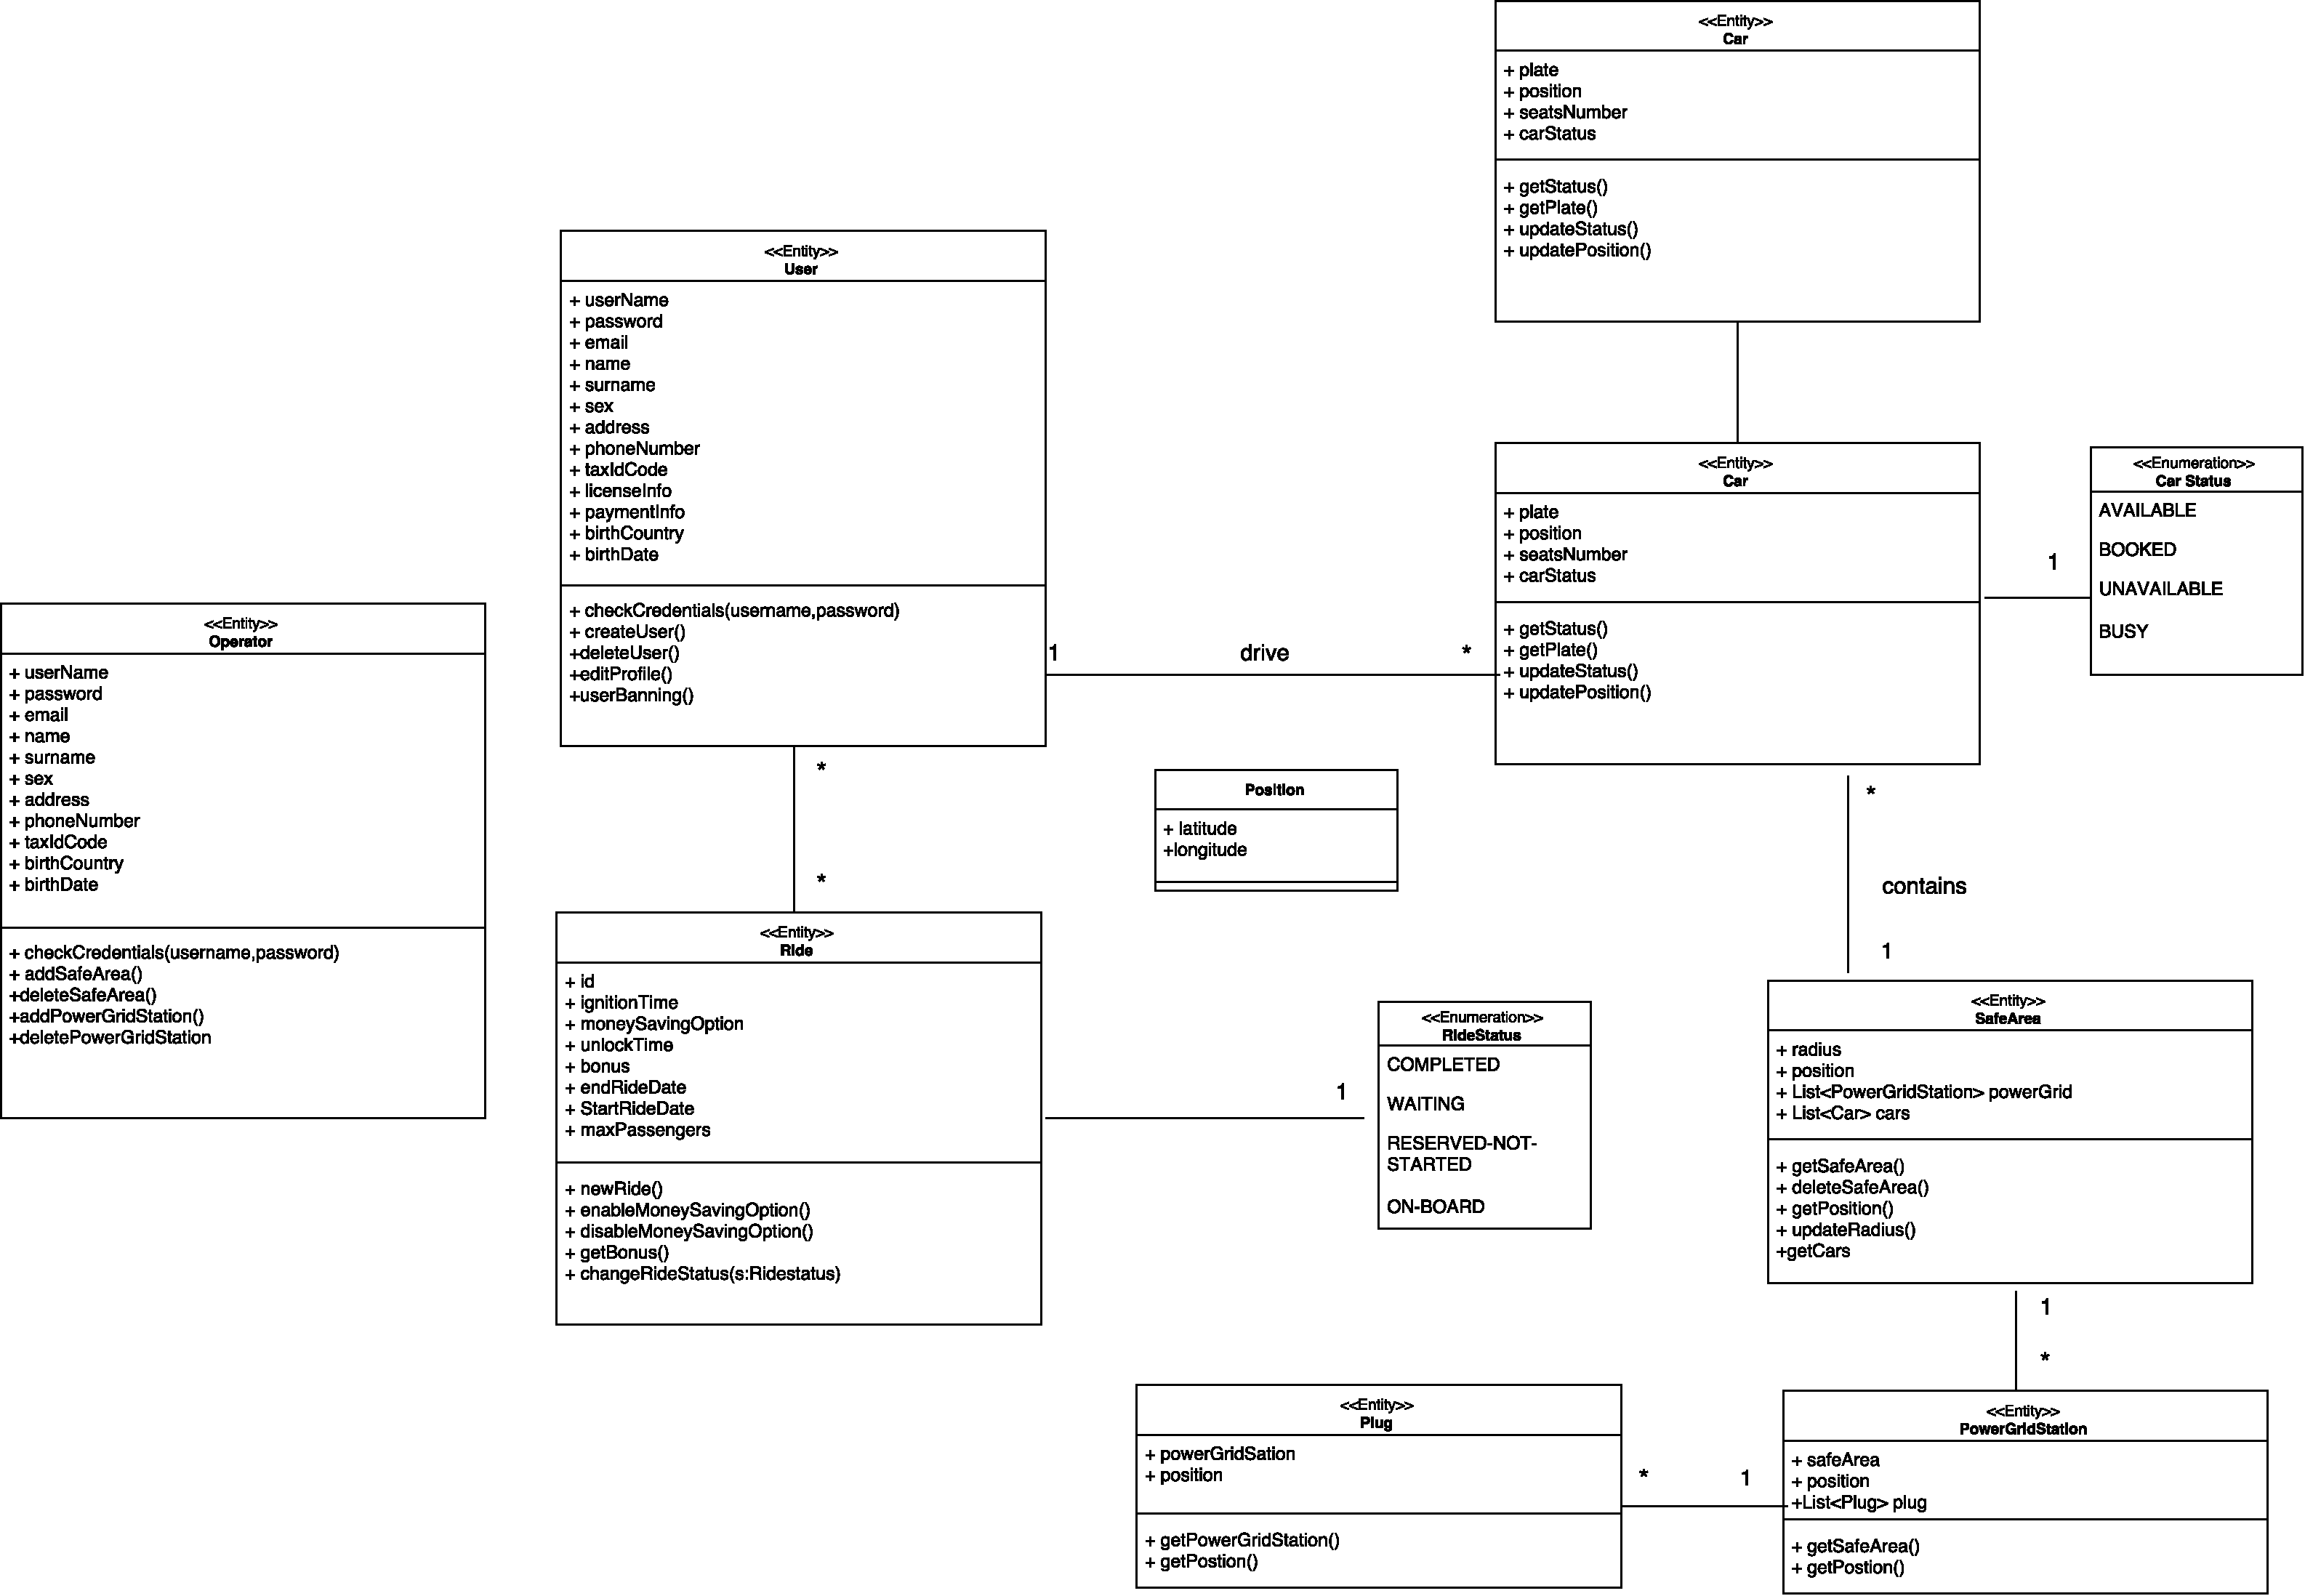
\includepdf{architectural_design/Architecture_Diagrams/EntityBeans.pdf}
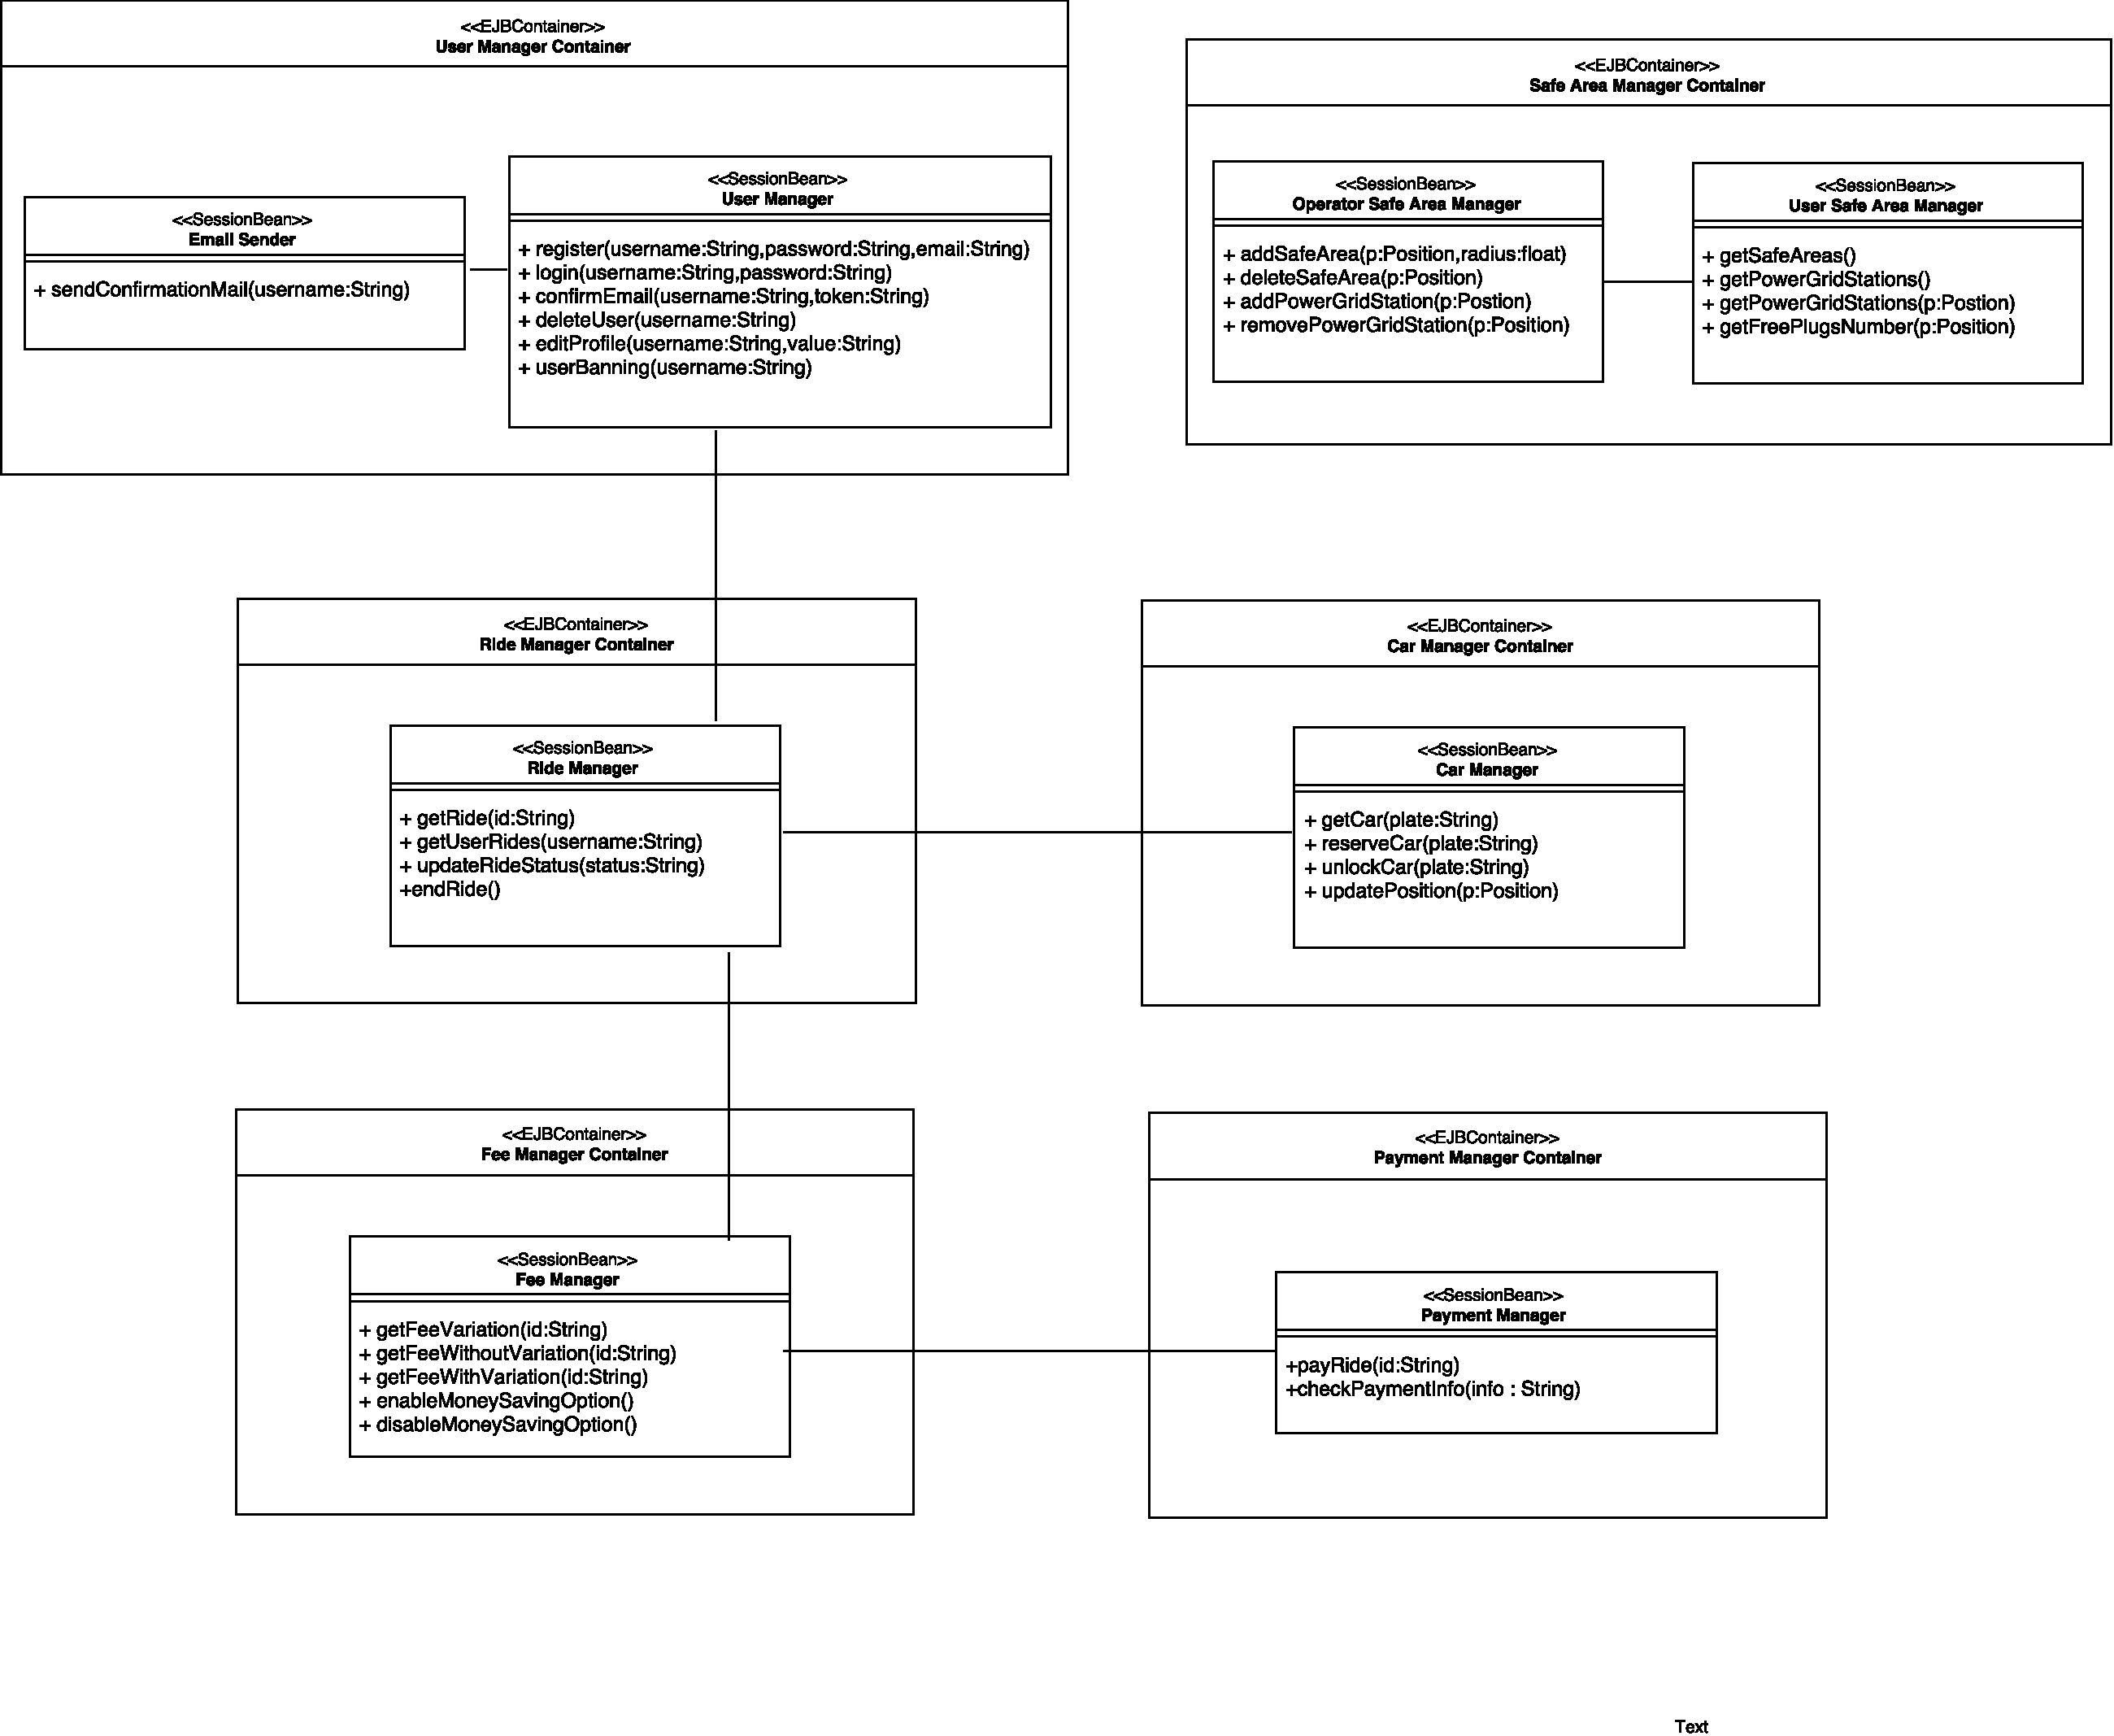
\includepdf{architectural_design/Architecture_Diagrams/SessionBeans.pdf}

\subsection{User Manager}
This bean manages all the user management features: user registration, user login user deletion, profile editing and user banning.
It also provides a function to confirm the email address provided by the user with the token sent by email.

This bean also communicates with two external systems:
\begin{itemize}
\item External Payment System, that checks that the payment information provided by the user are correct and handle the payment process;
\item External System for Driving License Validation, that checks the driving license of the user during the registration process.
\end{itemize}

\subsection{Car Manager}
This bean manages manages all the car's features: get car, reserve car, unlock car and update position.
In this way it keeps references and update all the informations about the car, including the maximum number of passengers the battery level and the numbers of seats.
It also provides a function to handles the changes in the status of the car.

This bean also communicates with the External System for Maintainers, because the bean signals the unavailable cars to it.

\subsection{Ride Manager}
This bean manages all the ride features:create new ride, get ride,get user's ride and end ride.
It provides functions that return all the rides informations like the number of passenger on the car,the unlock time and the user that has reserved the car.

\subsection{Fee Manager}
This bean manages all the functionalities about the fee of the ride: calculate fee variation, calculate fee with variation and calculate the fee without variation.
It handles all the information about the bill that the user has to pay and apply discounts when it is necessary.

\subsection{Safe Area Manager}
This bean allows the operator to manage the safe area and provides functions to add a new safe area and to delete it. It also provides function to add and delete a power grid station in a specific position.
Besides it offers also some function available also to the user that allows him/her to know the safe areas and power grid stations positions.

\subsection{Payment Manager}
This bean provide a function to pay the ride and another one to check the payment information provided by the user thanks to an external system of payment information validation.